
\documentclass{article}

% Language setting
% Replace `english' with e.g. `spanish' to change the document language
\usepackage[english]{babel}

% Set page size and margins
% Replace `letterpaper' with `a4paper' for UK/EU standard size
\usepackage[letterpaper,top=2cm,bottom=2cm,left=3cm,right=3cm,marginparwidth=1.75cm]{geometry}

% Useful packages
\usepackage{amsmath}
\usepackage{graphicx}
\usepackage[colorlinks=true, allcolors=blue]{hyperref}
\usepackage{wrapfig}


\title{\Large \textbf{Notes on Statistical Mechanics}}
\author{Riddhiman Bhattacharya}

\begin{document}
\maketitle


\section{\Large Introduction}
\large
Statistical physics is a powerful framework that enables us to understand and predict the collective behavior of large systems by using statistical methods and concepts like probability, entropy, and equilibrium. It plays a fundamental role in our understanding of many physical processes and has wide-ranging applications across scientific disciplines.

\section{Thermodynamics}
Thermodynamics is a branch of physics that provides a phenomenological description of macroscopic systems in thermal equilibrium. It deals with the macroscopic properties of matter, such as temperature, pressure, and energy, without explicitly considering the microscopic details. Thermodynamics focuses on the principles and laws that govern the relationships between these properties, enabling the prediction and analysis of system behavior.

\subsection{\Large Some Important Concepts under Thermodynamics}
\subsubsection{\large System}
In the context of thermodynamics, a "system" refers to the portion of the universe under consideration or study. It can be any distinct and well-defined region or object that is the subject of analysis. The system is often separated from its surroundings, which include everything outside of the system boundaries.

In thermodynamics, systems are classified into different types based on their interactions with their surroundings. The three primary types of systems are:

\begin{itemize}
\item \textbf{Closed System:} allows \textbf{heat transfer but do not allow transfer of matter across it}
\item \textbf{Open System:} has at least one wall that separates it from another thermodynamic system
\begin{itemize}
    \item \textbf{\textit{heat flows and it can't maintain temperature difference across itself}}.
    \item \textbf{\textit{the wall being permeable to at least one chemical substance, as well as to radiation; such a wall}}.
\end{itemize}
\item \textbf{Isolated System} Adiabatic wall (isolated system): does not allow \textbf{heat} or \textbf{chemical substances (mass transfer)} to pass across it.

\textit{An essential prerequisite for the measurability of energy is the existence of walls that do not permit the transfer of
energy in the form of heat.}
\end{itemize}

\subsection{Laws of Thermodynamics}

The laws of thermodynamics, which describe the behavior of macroscopic systems, are derived from empirical observations and experiments. These laws, including the conservation of energy, the increase of entropy, and the impossibility of reaching absolute zero temperature, provide fundamental principles for understanding and analyzing thermal systems.
On the other hand, statistical mechanics aims to establish a connection between the macroscopic laws of thermodynamics and the microscopic behavior of individual particles. By applying concepts from classical or quantum mechanics, statistical mechanics seeks to derive the macroscopic laws starting from the microscopic equations.
In classical statistical mechanics, the behavior of a large ensemble of particles is described using probability distributions and statistical averages. This approach allows for the calculation of macroscopic quantities, such as temperature and pressure, based on the properties of individual particles.
In quantum statistical mechanics, the principles of quantum mechanics are applied to describe the statistical behavior of quantum systems. Quantum statistical mechanics provides a framework for understanding the thermodynamic properties of systems composed of quantum particles, such as atoms and molecules.
By connecting the microscopic behavior of particles to the macroscopic laws of thermodynamics, statistical mechanics provides a theoretical foundation for explaining and predicting the thermodynamic properties of materials and systems. It allows us to bridge the gap between the microscopic and macroscopic descriptions of physical phenomena, providing a deeper understanding of the underlying mechanisms governing thermodynamic processes.
\subsection{Zeroth Law}
If two systems, A and B, are separately in equilibrium with a third system, C, then they are also in equilibrium with one
another.
\begin{itemize}
    \item implies the existence of an important state function, the empirical temperature $ \Theta$

  

  


\end{itemize}
Let $ \{X1, X2, \ldots\} $ be state functions of system $X$. $X$ can be $A,B$ and $C$

When 2 systems are in equilibrium there is a
constraint between their coordinates
  $$f_{AC}(A_1, A_2, \ldots ; C_1, C_2, \ldots) = 0$$
  $$f_{BC}(B_1, B_2, \ldots ; C_1, C_2, \ldots) = 0$$
 assuming that we can obtain an explicit function of $C_1$.

 $$C_1 = F_{AC}(A_1, A_2, \ldots ; C_2,\ldots)$$
 $$C_1 = F_{BC}(B_1, B_2, \ldots ; C_2,\ldots)$$
 $$\Rightarrow F_{AC}(A_1, A_2, \ldots ; C_2,\ldots) = F_{BC}(B_1, B_2,\ldots ; C_2,\ldots)$$

Now the \textbf{Zeroth law} states that we can always eliminate $\{C_1, C_2, \ldots\}$ from the equation and get

$$f_{AB}(A_1, A_2, \ldots ; B_1, B_2, \ldots) = 0$$

\subsection{First Law of Thermodynamics}
The \textbf{first law of thermodynamics}, also known as the \textbf{law of energy conservation}, states that \textit{energy cannot be created or destroyed in an isolated system}. The total energy of a system remains constant; it can only be transferred or converted from one form to another.

$$dE = dQ + dW$$

\begin{itemize}
    \item Based on the experimental fact that if we adiabatically isolate a system then the work done only depends on the final
and initial states
     \item $dE$ is an exact differential but $dQ$ and $dW$ are not.
\end{itemize}
\subsection{Second Law of Thermodyanmics}
\begin{itemize}
    \item \textbf{Kelvin's Statement:} \textit{No process is possible whose sole result is the complete conversion of heat into work.}
    \item \textbf{Clausius's Statement:} \textit{No process is possible whose sole result is the transfer of heat from a colder to a hotter body.}
    
    \item \textbf{Reversible Process:} \textit{Direction of reaction can be reversed by infinitesimal changes in some properties of the surroundings, such as pressure, temperature.}
    \item \textbf{Cyclic Process:} \textit{returns to the initial state.}
    
    \item \textbf{Quasi-static Process:} \textit{It happens slowly enough for the system to remain in internal physical (but not necessarily chemical)
thermodynamic equilibrium.}


\end{itemize}
\begin{enumerate}
    \item  All reversible processes are cyclic but not vice versa.
    \item All reversible processes are quasi-static but not vice versa.
\end{enumerate}

    


\subsubsection{Concept of Entropy}
One of the key concepts in statistical physics is entropy, which measures the degree of disorder or randomness in a system. The second law of thermodynamics states that entropy tends to increase in an isolated system. Statistical physics provides a microscopic understanding of this law by linking entropy to the underlying probabilities of different states.
\textbf{Clausius's Statement:}For any cyclic transformation (reversible or not), $\oint \frac{{dQ}}{{T_{\text{surr}}}} \leq 0 $ where $dQ$ is the heat increment supplied to the system at temperature T.
The equality holds only for reversible processes. 
\textbf{all reversible processes with same initial and final points will both have same change in entropy. If we consider only only reversible paths then entropy behaves like a state function. So,
for any reversible path}
$$dQ=TdS$$
$$dE = TdS + \sum_{i} J_i dx_i$$

\textbf{Generalised Inequality of Clausius} states that for an infinitesimal change in entropy $S$ applies not only to cyclic processes, but to any process that occurs in a closed system.
$$dS_{\text{sys}} \geq \frac{\delta Q}{{T_{\text{surr}}}}$$

 
 \subsection{Third Law}
 
\textit{\large The third law of thermodynamics, also known as the Nernst heat theorem, states that as the temperature of a system approaches absolute zero (0 kelvin) ($T \to 0$), the entropy of the system ($S \to 0 $) tends to a minimum value or approaches zero }
$$\lim_{{T \to 0}} S(X, T) = S(X, 0) = 0 $$

\subsection{Ideal Gas}
\subsubsection{Joule's Free Expansion Experiment}
\large 
Joule's free expansion experiment was conducted by \textbf{James Joule} in the 1840s to study the \textit{behavior of gases during an unrestrained expansion}. The experiment was designed to investigate the relationship between the volume change and temperature change of a gas undergoing a free expansion.
In Joule's experiment, a gas is confined within an insulated chamber fitted with a partition. The partition has a small opening or porous plug that allows the gas to escape into an evacuated chamber. Initially, the gas is in thermal equilibrium with the surroundings.






\begin{wrapfigure}{l}{0.5\textwidth}
  \begin{center}
    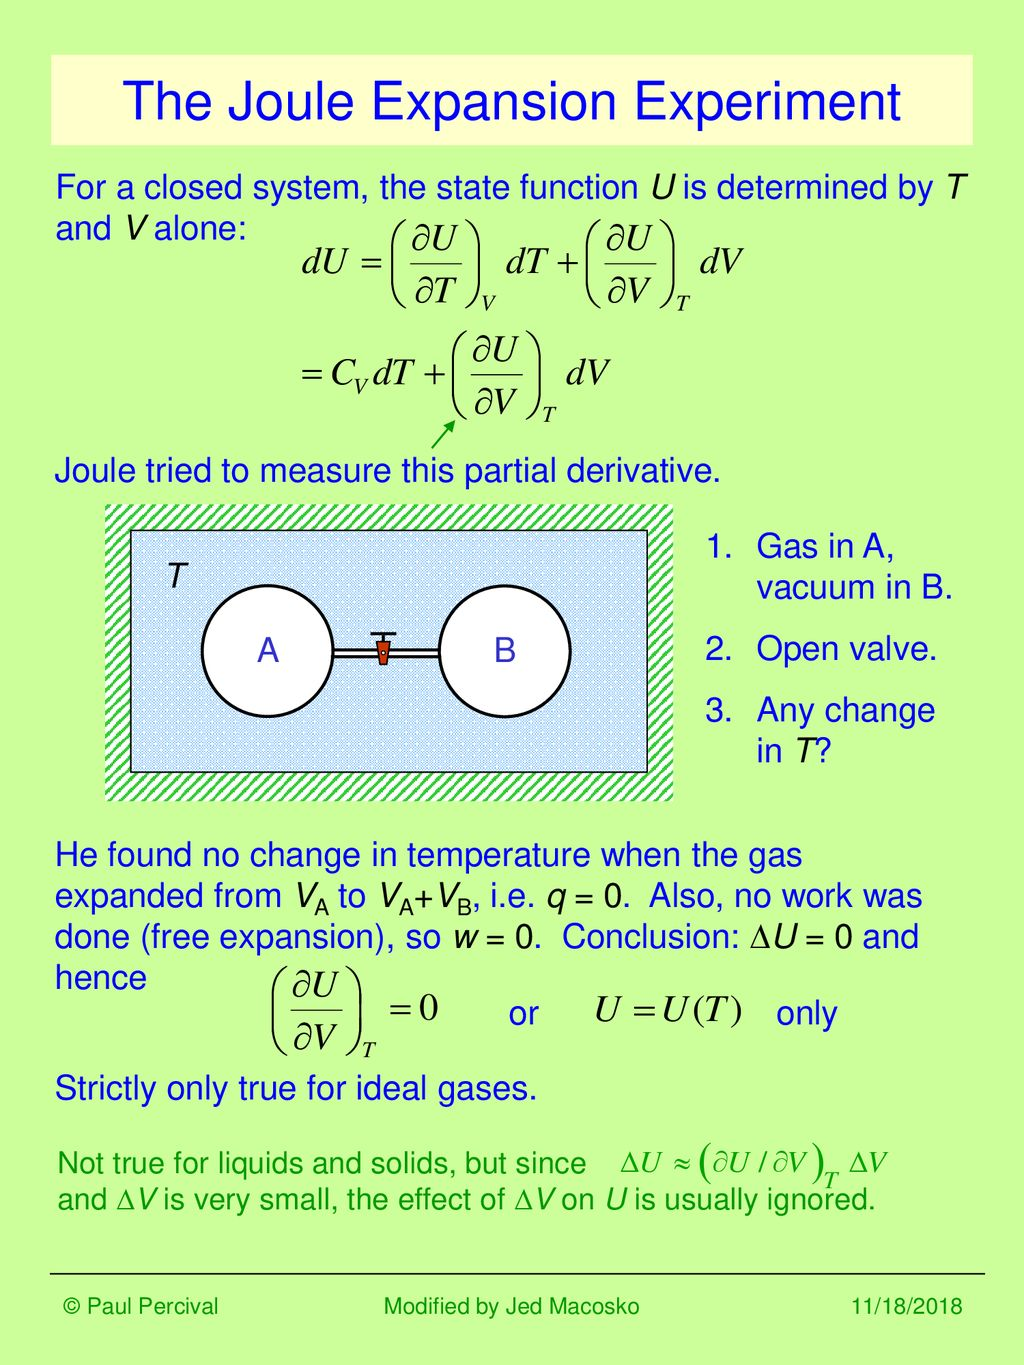
\includegraphics[width=0.35\textwidth]{JOULE'S FREE EXPANSION Experiment.jpg}
  \end{center}

\end{wrapfigure}


To perform the experiment, the partition is suddenly removed, allowing the gas to expand freely into the evacuated chamber. Since the expansion occurs rapidly, there is no time for heat exchange between the gas and the surroundings, making it an adiabatic process. As a result, the expansion is considered reversible and the internal energy of the gas remains constant.
During the free expansion, Joule observed that the temperature of the gas decreased. This decrease in temperature was explained by the fact that the energy required for the expansion is obtained from the internal energy of the gas itself. As the gas expands, it does work against its own internal pressure, leading to a decrease in temperature due to the reduction in kinetic energy of the gas molecules.

\subsubsection{\large Ideal Gas}
According to \textbf{Joule's Free Expansion Experiment} $E(V, T) = E(T)$

$$\kappa_T = \frac{1}{P}$$
$$C_P - C_V = Nk_B$$
$$\mu = -\left(\frac{{\partial S}}{{\partial N}}\right)_{E,V}T=T k_B \ln[\frac{V}{N}\left(\frac{{4\pi m E}}{{3N}}\right)^{\frac{3}{2}})]$$

$$\Omega(N, E, V)
=\frac{{V^N}}{{N!}}\frac{{2\pi^{3N/2}}}{{(3N/2 - 1)!}}(2mE) \Delta R$$

$$ S=N k_B \ln[\frac{V}{N}\left(\frac{{4\pi m E}}{{3N}}\right)^{\frac{3}{2}}] $$
$$\frac{S}{k_B N} = \ln \left[ \frac{V}{N} \left( \frac{{4\pi m}}{{3h^2}} \frac{U}{N} \right)^{\frac{3}{2}} \right] + \frac{5}{2} $$


$$\lambda(T) = \frac{h}{{\sqrt{2\pi m k_B T}}}$$


\subsection{Gibbs-Duhem Relation}
The Gibbs-Duhem relation is a consequence of the fundamental principles of thermodynamics and holds for any system in thermodynamic equilibrium, regardless of the specific details of the system or the interactions between its constituents. It serves as a powerful tool for analyzing and understanding the thermodynamic properties of complex systems.
It establishes a relationship between the partial derivatives of intensive variables in a thermodynamic system. It is named after \textbf{Josiah Willard Gibbs} and \textbf{Pierre Duhem}, who independently derived this relation.

The Gibbs-Duhem relation states that \textit{in a system at equilibrium, the partial derivatives of intensive variables with respect to the extensive variables satisfy the equation}
\large
$$\sum_{i} n_{i} \, d\mu_{i}=0$$

Simply, the Gibbs-Duhem relation states that the \textbf{sum of the changes in the chemical potentials of all components in a system is zero. This equation reflects the fact that in a thermodynamic system, there is a conservation of the number of particles, and any change in the chemical potential of one component must be compensated by changes in the chemical potentials of other components.}

$$dE = T \, dS + J \cdot dx + \mu \cdot dN $$
$$E(\lambda S, \lambda x, \lambda N) = \lambda E(S, x, N)$$

$$\frac{{\partial E}}{{\partial S}} \Bigg|_{(x, N)}+\sum \frac{{\partial E}}{{\partial x_i}} \Bigg|_{S, x_j \neq x_i, N}+\sum \frac{{\partial E}}{{\partial N_\alpha}} \Bigg|_{S,x,N_\beta \neq \alpha} N_\alpha=E(S, x, N)
$$



Now from the Equation 1, we substitute the partial derivatives
$$E = TS + J \cdot x + \mu \cdot N$$
$$SdT + x \cdot dJ + N \cdot d\mu = 0$$



The Gibbs-Duhem relation is particularly useful in understanding phase equilibrium and the behavior of mixtures. It provides a constraint on the relationships between intensive variables, such as temperature, pressure, and chemical potential, in a multi-component system.

\section{Probablity}
At the heart of statistical physics lies the concept of probability. Instead of focusing on the precise details of individual particles, statistical physics examines the statistical distribution of their properties. This statistical approach allows us to make predictions about the macroscopic behavior of a system based on its microscopic constituents.
We'll discuss these in a separate document "Probability"

\section{Classical Statistical Mechanics}
In classical statistical mechanics, the system is described by a set of classical variables such as position and momentum. The state of the system is characterized by a probability distribution function, often referred to as the phase space distribution, which describes the likelihood of finding the system in a particular configuration of the classical variables.

The fundamental principles of classical statistical mechanics, such as the \textbf{Ergodic hypothesis} and the principle of equal a \textbf{Priori probabilities}, allow for the calculation of various thermodynamic properties of the system. These properties include the equilibrium distribution of particles, energy, temperature, entropy, and other macroscopic observables.

$$S_{n-1} = \frac{{n\pi^{n/2}}}{{\Gamma((n/2)+1)}} R^{n-1}=\left[\frac{{2\pi^{n/2}}}{{\Gamma(n/2+1)}}\right] R^{n-1} $$

$$\Gamma(x + 1) = x!$$
$$\Gamma\left(\frac{1}{2}\right) = \left(-\frac{1}{2}\right)! = \sqrt{\pi}$$


\subsection{Ergodic Hypothesis}
The ergodic hypothesis is a fundamental concept in statistical mechanics that relates the time average of a physical observable to its ensemble average. The hypothesis states that in an ergodic system, the time spent by a system in a particular region of its phase space is proportional to the measure (volume) of that region.
In other words, the ergodic hypothesis assumes that over long periods of time, a system explores and visits all accessible states in its phase space in a statistically representative manner. This implies that the time average of a physical quantity, such as energy or momentum, taken over a sufficiently long time period is equal to the ensemble average of that quantity, which is calculated by averaging over all possible states of the system.

\textbf{\textit{For a dynamical system described by its phase space coordinates (q, p), the ergodic hypothesis states that an observable quantity A(q, p) can be time-averaged over a sufficiently long time period and be equivalent to its ensemble average over all possible states of the system.}}
Mathematically, the time average of the observable A is given by:

$$\langle A \rangle_T = \lim_{{T\to\infty}} \left(\frac{1}{T} \int_0^T A(q(t), p(t)) dt\right)$$

where $q(t)$ and $p(t)$ represent the trajectory of the system in phase space over time.

\subsection{Ensembles}
Ensembles in statistical mechanics refer to different probability distributions that describe -the statistical properties of a system in equilibrium. These ensembles provide a framework for studying the behavior of a large number of particles and their interactions.
\begin{itemize}
    \item \textbf{In the thermodynamic limit $N \rightarrow \infty
$ all these ensembles are in fact equivalent. They describe the same systems but
through different variables}
\end{itemize}
\textbf{Key Point:} For example in the grand canonical $N$ is not fixed. But the probability of $N$ is almost a delta function and
average=most probable. This logic won't for Maxwell Boltzmann distribution because it is completely different. There
you are talking about single particle not an ensemble. It is microscopic quantity not macroscopic


\subsubsection{Microcanonical Ensemble:} It describes an isolated system with fixed total energy, volume, and particle number. In this ensemble, all accessible microstates with the same energy are equally likely.
\begin{itemize}
    \item macrostate $M \equiv (E, x)
$
    \item $(E,V,N)$ is constant among microstates and parametrize the system.
    \item Finding $\Omega(E, x)$ and $S(E, x) = k_B \log \Omega(E, x)
$ and using entropy we can find any other function

\end{itemize}
\subsubsection{Gibb's Paradox:} 
For an Ideal Gas
$$\Omega(N, E, V)
=\frac{{V^N}}{{N!}}\frac{{2\pi^{3N/2}}}{{(3N/2 - 1)!}}(2mE) \Delta R$$
\begin{itemize}
    \item Ideal gas in \textit{not consistent with classical mechanics} as the entropy is not extensive.

    \item Once we use the the fact that the particles are identical from quantum mechanics then the inconsistency is gone.
\end{itemize}

\subsubsection{Canonical Ensemble:} It describes a system in contact with a heat reservoir at a fixed temperature. The energy of the system is allowed to fluctuate, but the average energy is fixed. This ensemble is suitable for describing systems at constant temperature.

$$F(T, x) = -k_BT \ln Z(T, x)$$
$$p(T, x)(\mu) = \frac{e^{-\beta H(\mu)}}{Z(T, x)}$$
$$Z(T, x) = \sum_{\mu} e^{-\beta H(\mu)} = \sum_{\epsilon} e^{-\beta F(E)} \approx e^{-\beta F(E^*)}$$
$$p(E) = \sum_{\mu} p(\mu) \delta(H(\mu) - \epsilon) = \Omega(E) e^{-\beta E}/Z = \frac{1}{Z}\exp\left[-\frac{F(\epsilon)}{k_BT}\right]
$$
$$E = \langle H \rangle = \sum_{\mu} H(\mu)e^{-\beta H(\mu)}/Z = -\frac{1}{Z}\left(\frac{\partial}{\partial\beta}\right)\sum_{\mu} e^{-\beta H} =-\frac{\partial \ln Z}{\partial \beta}$$
\begin{itemize}
    \item macrostate $M \equiv (T, x)
$
\item $dW = 0$ but
$dQ \neq 0$
\item $(T,V,N)$ constant among microstates and parametrize the system.
\item thermodynamic limit of $N \rightarrow \infty$
, the canonical energy probability is so sharply peaked around the average energy that
the ensemble becomes essentially indistinguishable from the microcanonical ensemble at that energy.


\end{itemize}




\subsubsection{Grand Canonical Ensemble:} It describes a system in contact with a heat reservoir and a particle reservoir, allowing both energy and particle exchange with the reservoirs. The average energy and particle number can fluctuate, but their average values are fixed. This ensemble is used to describe systems at constant temperature and chemical potential.
\begin{itemize}
    \item macrostate $M \equiv (T, \mu, x)
$
\item $dW \neq 0$, $dW \neq 0$


\item $(T, V, \mu)$ is constant among microstates and parametrize the system.
$$Q(T, \mu, x) = \sum_{\mu}S e^{\left[\beta\mu N(\mu S)-\beta H(\mu S)\right]}$$

$$G(T, \mu, x) = E - TS - \mu N = -k_BT \ln Q$$

$$\langle N \rangle = \frac{\partial \ln Q}{\partial (\beta\mu)}$$



\end{itemize}

\subsubsection{Gibb's Canonical Ensemble}
\begin{itemize}
    \item macrostate $M \equiv (T, J)
$
\item $dW \neq 0$, $dW \neq 0$
\item $(N, P, T)$ is constant among microstates and parametrize the system.

$$Z(N, T, J) = \sum_{(\mu_S, x)} e^{\left(\beta J \cdot x - \beta H(\mu_S)\right)}$$

$$G(N, T, J) = -k_BT \ln Z$$
$$H = \langle H - x \cdot J \rangle = -\frac{\partial \ln Z}{\partial \beta}$$



\end{itemize}




\section{Quantum Statistical Mechanics}

\textbf{Quantum statistical mechanics} is a branch of physics that combines principles from quantum mechanics and statistical mechanics to describe the behavior of quantum systems in thermal equilibrium. It provides a framework for studying the statistical properties of particles and their interactions at the quantum level.
In quantum statistical mechanics, \textit{the state of a system is described by a density operator or density matrix, which represents the probabilities of different quantum states of the system}. The density matrix evolves in time according to the \textbf{Schrödinger equation} or the \textbf{von Neumann equation}, depending on whether the system is in a closed or open quantum system.
The theory allows for the calculation of various properties of quantum systems, including the calculation of average values of observables, fluctuations, and thermodynamic quantities. 

\subsection{Density Matrix}
\large
$$\rho = \sum_{j} p_j \vert \psi_j \rangle \langle \psi_j \vert$$
$$\langle A \rangle = \text{tr}(\rho A)$$
$$i\hbar \frac{{\partial \rho}}{{\partial t}} = [H, \rho] $$


The criterion for determining whether a density matrix describes a pure or mixed state is based on the properties of the trace and the von Neumann entropy.

\subsubsection{\textbf{Trace Criterion:}} The trace of a density matrix $\rho$  represents the sum of its diagonal elements. \textbf{If the state is pure, meaning it is described by a single quantum state, the trace of 
$\rho$  will be equal to $1$.} This is because in a pure state, the density matrix has only one non-zero eigenvalue, corresponding to the probability of being in that particular state. On the other hand, \textbf{if the state is mixed, meaning it is a statistical mixture of multiple quantum states, the trace of $\rho$ will be less than 1}. This is because, in a mixed state, the density matrix has multiple non-zero eigenvalues, representing the probabilities of different states in the mixture.




 \subsubsection{\textbf{Von Neumann Entropy Criterion:}} The von Neumann entropy is a measure of the amount of information or uncertainty in a quantum state. \textbf{For a pure state, where there is no uncertainty, the von Neumann entropy is zero}. This is because in a pure state, the density matrix has only one non-zero eigenvalue, resulting in a simple and deterministic state. '
 
 \begin{align*}
\rho = \vert \psi \rangle \langle \psi \vert \Rightarrow \rho = \rho^2
\end{align*}

 
 Conversely, \textbf{for a mixed state, where there is inherent uncertainty due to the statistical mixture of states, the von Neumann entropy is strictly positive}. This is because in a mixed state, the density matrix has multiple non-zero eigenvalues, indicating a greater degree of uncertainty or mixedness in the state.

These two criteria provide equivalent ways to determine whether a density matrix represents a pure or mixed state. 
The trace criterion examines the sum of diagonal elements, while the von Neumann entropy criterion considers the overall entropy of the state. Both criteria can be used to assess the nature of the quantum state described by a density matrix.
\subsection{Fugacity}

The concept of fugacity(Z) is used to describe the \textbf{deviation of the quantum mechanical behavior of particles from classical behavior}. Fugacity is a thermodynamic quantity that relates to the concentration or density of particles in a quantum system.
The fugacity is determined by considering the energy levels and quantum states available to the particles in the system. By accounting for the effects of quantum indistinguishability and quantum statistics, the fugacity factor provides a more accurate description of the particle density in quantum systems compared to classical thermodynamics.

$$Z = e^{\beta\mu}$$



The concept of fugacity is particularly relevant in studying gases, such as Bose-Einstein condensates and Fermi gases, where quantum effects dominate at low temperatures



\section{Microcanonical Ensemble}


$$\rho(E) = \frac{\delta(H - E)}{\Omega(E)}$$

$$n|\rho|m⟩ = \sum_\alpha p_\alpha \langle n | \Psi_\alpha \rangle \langle \Psi_\alpha | m \rangle = \begin{cases} \Omega & \text{if } E_n = E \text{ and } m = n\\ 0 & \text{if } E_n \neq E \text{ or } m \neq n \end{cases}$$




\section{Canonical Ensemble}

$$\rho(\beta) = \frac{\exp(-\beta H)}{Z(\beta)}$$
$$Z = \text{tr}(e^{-\beta H}) = \sum_n e^{-\beta E_n}$$



\section{Grand Canonical Ensemble}

Here we are expressing it in terms of canonical partition function

$$\rho(\beta, \mu) = \frac{e^{-\beta H + \beta \mu N}}{Q}$$

$$Q(\beta, \mu) = \text{tr}(e^{-\beta H + \beta \mu N}) = \sum_{N=0}^\infty e^{\beta \mu N} Z_N(\beta)$$











\end{document}
